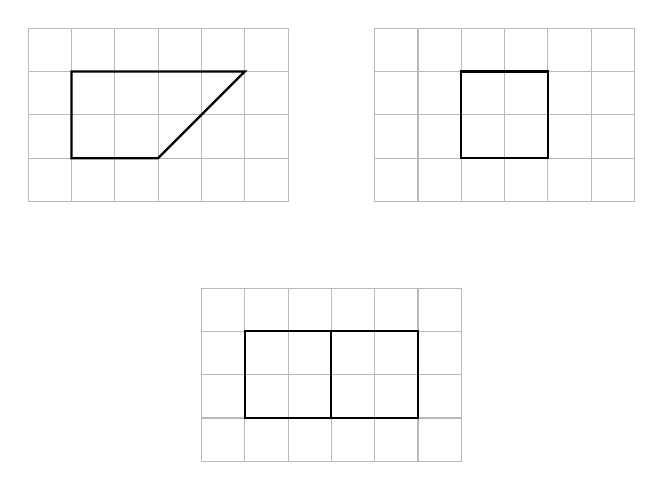
\begin{tikzpicture}[scale=0.55]
\foreach \x/\y in {0/0,8/0,4/-6} {
  \draw[gray!55,thin] (\x,\y) rectangle ++(6,4);
  \foreach \i in {1,...,5} {\draw[gray!55,thin] (\x+\i,\y) -- (\x+\i,\y+4);}
  \foreach \j in {1,2,3} {\draw[gray!55,thin] (\x,\y+\j) -- (\x+6,\y+\j);}
}
\draw[thick] (1,1) -- (3,1) -- (5,3) -- (1,3) -- cycle;
\draw[thick] (10,1) rectangle (12,3);
\draw[thick] (5,-5) rectangle (9,-3);
\draw[thick] (7,-5) -- (7,-3);
\end{tikzpicture}
